
\lecture{Lecture - 24\hfill 23 Oct 24, Wed}

A way to quantify how connectd a graph is, is to measure how quickly the random walk on the graph `mixes.'
\begin{definition}
	Given a simple grap $G = (V,E),$ a random walk on $G$ is a sequence $(X_0, X_1, \dotsc)$ of $G$ valued random variables, such that
	$$P\left\{ X_{n+1} = j \, | \, X_n = i \right\} 
	= \begin{cases}
	0 & \text{ if } j \not \in N(i) \\
	\frac{1}{d(i)} & \text{ if } j \in N(i) \\
	\end{cases}.$$
\end{definition}
\begin{theorem}
	If the graph $G$ is simple and connected, then
	$ \lim_{n \to \infty} P(X_n = i) = \frac{1}{ \lvert V \rvert}.$
\end{theorem}
\begin{remark}
	In probabilitistic language, the random walk on a graph is a 
	Markov chain, and the stationary, or equilibrium, distribution
	is the uniform distribution on $V.$
\end{remark}
A bottleneck is a small number of edges required to disconnect $G.$
Presence of a bottleneck prevents fast mixing.
The speed of convergence of $P\left\{ X_n = i \right\}$ to $\frac{1}{ \lvert V \rvert}$ is intimately connected to 


\begin{figure}[h]
\centering
	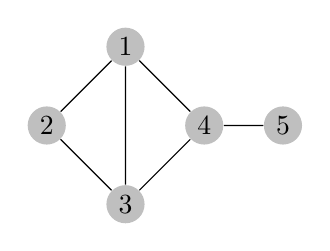
\begin{tikzpicture}
		\tikzstyle{vertex}=[circle,fill=black!25,minimum size=12pt,inner sep=2pt]
		\node[vertex] (g_1) at (3,2) {1};
		\node[vertex] (g_2) at (2,1) {2};
		\node[vertex] (g_3) at (3,0) {3};
		\node[vertex] (g_4) at (4,1) {4};
		\node[vertex] (g_5) at (5,1) {5};
		\draw (g_1) -- (g_2) -- (g_3) -- (g_4) -- (g_1)
			(g_4) -- (g_5) (g_1) -- (g_3);
	\end{tikzpicture}
\end{figure}

$$ A = \begin{pmatrix}
     0    &     1    &     1    &     0    &     0    \\
     1    &     0    &     1    &     1    &     0    \\
     1    &     1    &     0    &     1    &     0    \\
     0    &     1    &     1    &     0    &     1    \\
     0    &     0    &     0    &     1    &     0    \\
\end{pmatrix}$$
$$= \begin{pmatrix}
     2    &    -1    &    -1    &     0    &     0    \\
    -1    &     3    &    -1    &    -1    &     0    \\
    -1    &    -1    &     3    &    -1    &     0    \\
     0    &    -1    &    -1    &     3    &    -1    \\
     0    &    -1    &    -1    &     3    &    -1    \\
     0    &     0    &     0    &    -1    &     1    \\
\end{pmatrix}$$

We can represent an oriented or directed graph by
$$\overrightarrow{E} = \left\{ (a,b) \, : \, a
\text{ is the head of an edge } e \text{ and }
b \text{ is the tail of } e, 
\text{ for some } e \in E \right\}.$$

Given a graph $G = (V,E)$ on $n$ vertices, we can orient each edge in 2
ways, so we can orient it in $2^{ \lvert E \rvert}$ ways.
\begin{definition}
Given an orientation of $G,$ the oriented, or directed, incidence matrix
of $G$ is the $\lvert V \rvert \times \lvert E \rvert$ matrix $N$
defined by
$$N(v,e) = \begin{cases}
	1 & \text{ if } v \text{ is the head of } e \\
	-1 & \text{ if } v \text{ is the tail of } e \\
	0 & \text{ otherwise }  \\
\end{cases}.$$
\end{definition}
The graph
\begin{figure}[h]
\centering
	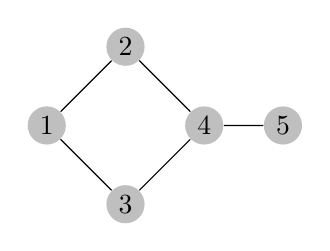
\begin{tikzpicture}
		\tikzstyle{vertex}=[circle,fill=black!25,minimum size=12pt,inner sep=2pt]
		\node[vertex] (g_1) at (0,1) {1};
		\node[vertex] (g_2) at (1,2) {2};
		\node[vertex] (g_3) at (1,0) {3};
		\node[vertex] (g_4) at (2,1) {4};
		\node[vertex] (g_5) at (3,1) {5};
		\draw (g_1) -> (g_2) -> (g_4) (g_1) ->(g_3) -> (g_4) -> (g_5);
	\end{tikzpicture}
\end{figure}
has the incidence matrix
$$ N = \begin{bmatrix}
    -1    &     -1    &     0    &     0    &     0    &     0    \\
     1    &     0    &     1    &     -1    &     0    &     0    \\
     0    &     1    &     -1    &     0    &     -1    &     0    \\
     0    &     0    &     0    &     1    &     1    &     -1    \\
     0    &     0    &     0    &     0    &     0    &     1    \\
\end{bmatrix}.$$
\begin{theorem}[]
	:et $G=  (V,E)$ be a simple graph. Then 
	\begin{enumerate}
		\item For any orientation of $G,$ if $N$ is the oriented
			incidence matrix, then
			$NN^T = L(G),$
		\item $L(G)$ is the positive semidefinite, that is, it
			is a real symmetric matrix with non negative
			characteristic values.
		\item The smallest characteristic value of $L(G)$ is
			$0,$ and its mulitiplicity equals the number
			of connected components of $G.$
	\end{enumerate}
\end{theorem}
